%\chapter{Einleitung}

\section{Einleitung}
\subsection{Forschungszentrum Informatik}
\label{sec:FZI}
\glqq Das FZI Forschungszentrum Informatik am Karlsruher Institut für Technologie ist eine gemeinnützige Einrichtung für Informatik-Anwendungsforschung und Technologietransfer. Es bringt die neuesten wissenschaftlichen Erkenntnisse der Informationstechnologie in Unternehmen und öffentliche Einrichtungen und qualifiziert junge Menschen für eine akademische und wirtschaftliche Karriere oder den Sprung in die Selbstständigkeit.\grqq{} \cite{FZI_info}

\subsection{Der Forschungsbereich ESS}
\label{sec:ESS}
\glqq Der Forschungsbereich \acf{ESS} beschäftigt sich mit innovativen Technologien, Entwurfsmethoden und Anwendungen für und von eingebetteten Systemen. Von modellbasierten Entwurfsmethoden und -werkzeugen über technologieorientierte Forschung bis hin zu anwendungsorientierten Forschungs- und Entwicklungsprojekten – wir gestalten und entwickeln praxistaugliche Anwendungen rund um eingebettete Systeme und evaluieren diese.

Die breite Technologie- und Systemkompetenz aus Elektronik, Software-Engineering, Optik und Optoelektronik, Mikrosystemtechnik und Sensorik ist ein Alleinstellungsmerkmal des Bereiches. Schwerpunkte der Arbeiten bilden dementsprechend vor allem stark interdisziplinäre, Technologieübergreifende Forschungsprojekte und Anwendungen von eingebetteten Systemen in der Automobilelektronik, der Industrieautomation und im Gesundheits- und Sozialwesen.

Der Bereich ESS deckt mit seinen verfügbaren Kompetenzen dabei das komplette Spektrum der Entwicklung eingebetteter Systeme und Cyber Physical Systems (CPS) mit heterogenen Komponenten aus Mikroelektronik, Mikrooptik, Mikromechanik und Telematik ab.\grqq{}  \cite{ESS}




\newpage
\subsection{Einleitung zum Projekt}
\label{sec:Porjekt}

"Nach einer Studie der Charité aus dem Jahr 2015 sterben in Europa jährlich 23.000 Menschen an den Folgen einer Infektion mit multiresistenten Keimen. Die Tendenz ist dabei steigend. Hauptursache für die Ausbreitung dieser Keime, wie beispielsweise MRSA, ist eine mangelnde Hygiene der Angestellten in den Versorgungseinrichtungen beim Umgang mit den Patienten. Gründe dafür liegen im fehlenden Problembewusstsein, der zu hohen Arbeitsdichte und damit verbundenem Zeitmangel und der mangelnden Qualifikation der beteiligten Pflegekräfte.\par
Ziel des Projekts HEIKE ist es neue, technikgestütze Möglichkeiten zu entwickeln, welche die behandelnden Mitarbeiter im Krankenhausumfeld bei Maßnahmen am Patienten unterstützen und dadurch deren Compliance in Bezug auf die Händedesinfektion erhöhen. \par
Die Grundlage bilden ein mobiler, vernetzter Desinfektionsspender sowie Augmented-Reality-Technik. Die Technologien werden in dem Projekt weiterentwickelt und in einem System integriert, welches automatisch die durchgeführten Handlungen am Patienten erkennt und basierend darauf zusätzliche Informationen zur Verfügung stellt. Schließlich werden die durchgeführten Maßnahmen automatisch im System dokumentiert, was den Verwaltungsoverhead für das operative Personal verringert." \cite{FZI_Projekt}
\begin{figure}[htb]
  \centering  
  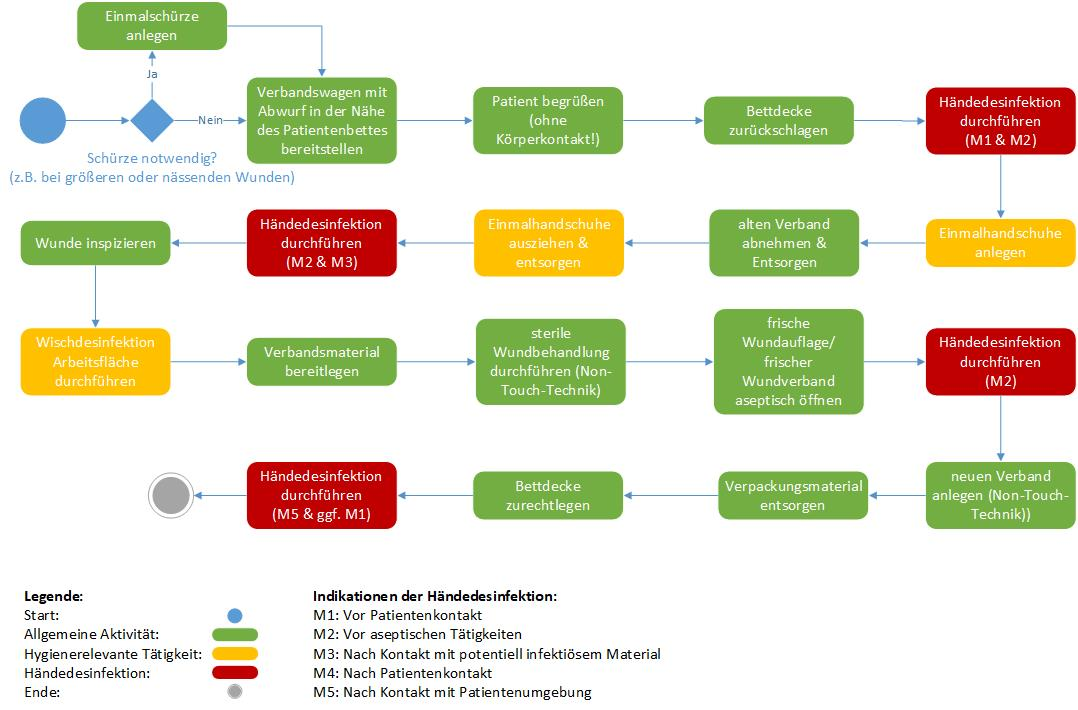
\includegraphics[scale=0.45]{img/Ablaufdiagramm_Verbandswechsel.jpg}
  \caption{Ablaufdiagramm Verbandswechsel \cite{AblauffdiagrammVerbandswechsel}}
  \label{fig:Ablaufdiagramm Verbandswechsel}
\end{figure}

\newpage
\subsection{Aufgabenstellung}
\label{sec:Aufgabenstellung}

Um diese Automatischen System, meist Deep Learning Methoden, zu trainieren braucht es sehr große Datenset und viele verschiedene Parameter, welche irgendwie nach groben ermessen und herum probieren vom Programmier ausgewählt werden. Diese Auszuwählen beansprucht sehr viel Zeit und Mühe. \par
Um dies dem Benutzer zu vereinfachen soll ein Konzept geschaffen werden, welches diese Vorgänge automatisiert und zusätzlich noch mit einen Optimierungsalgorithmus verbessert.Mit diesem Ansatz kann zum Beispiel die dimensionierung eines Netzes einfacher umgesetzt werden. Ein weiter Anwendungsfall ist die Hyperparameterauswahl. Mit hilfe diesem Werkzeug soll eine einfachere und bessere Auswahl der Hyperparameter erfolgen.\par Diese berechneten Werte sollen gespeicher und anschließend übersichtlich und intuitiv anzeigt werden. Wodurch die idealen Parameter herausbilden. Mit diesen Hyperparameter wird möglicherweise die Richtigkeit des Netzes erhöht, sodass dieses auf ein besseres Ergebnisse kommt. Dieses Werkzeug soll Konzeptioniert und Implementiert werden. Anschließend soll eine Evaluation und Auswertung über die mögliche Verbessung durchgeführt werden. 